\documentclass[12pt, a4 paper]{article}
\usepackage{babel}
\usepackage{graphicx, hyperref, xcolor, fancyhdr, amssymb, amsmath, pifont}
\usepackage{mathrsfs}
\usepackage[acronym, toc]{glossaries}
\usepackage{pdfpages}
\usepackage{svg}
\usepackage{algorithmic}
\usepackage[ruled, linesnumbered]{algorithm2e}

% \usepackage{times}

\hypersetup{
    colorlinks,
    linkcolor={red!60!black},
    citecolor={blue!80!black},
    urlcolor={blue!80!black}
}

% \pagestyle{fancy}
% \renewcommand\headrulewidth{.5pt}
% \fancyhead[L]{
%     V. Trélat
% }

% \fancyhead[C]{
%     \textbf{Verification in Isabelle/HOL of Hopcroft's algorithm for minimizing DFAs including runtime analysis}
% }

% \fancyhead[R]{
%     % Current section
%     \ifnum\c@secnumdepth>0
%         \thesection
% }


% Glossary

\makeglossaries

% \newacronym{tiaa}{TIAA}{This Is An Acronym}

\begin{document}

\begin{titlepage}
    \begin{center}
        \vfill
        
\includegraphics[height=1.5cm]{img/logoTUM.png}
        \hfill
        
\includegraphics[height=1.5cm]{img/logoartem.png}
        \hfill
        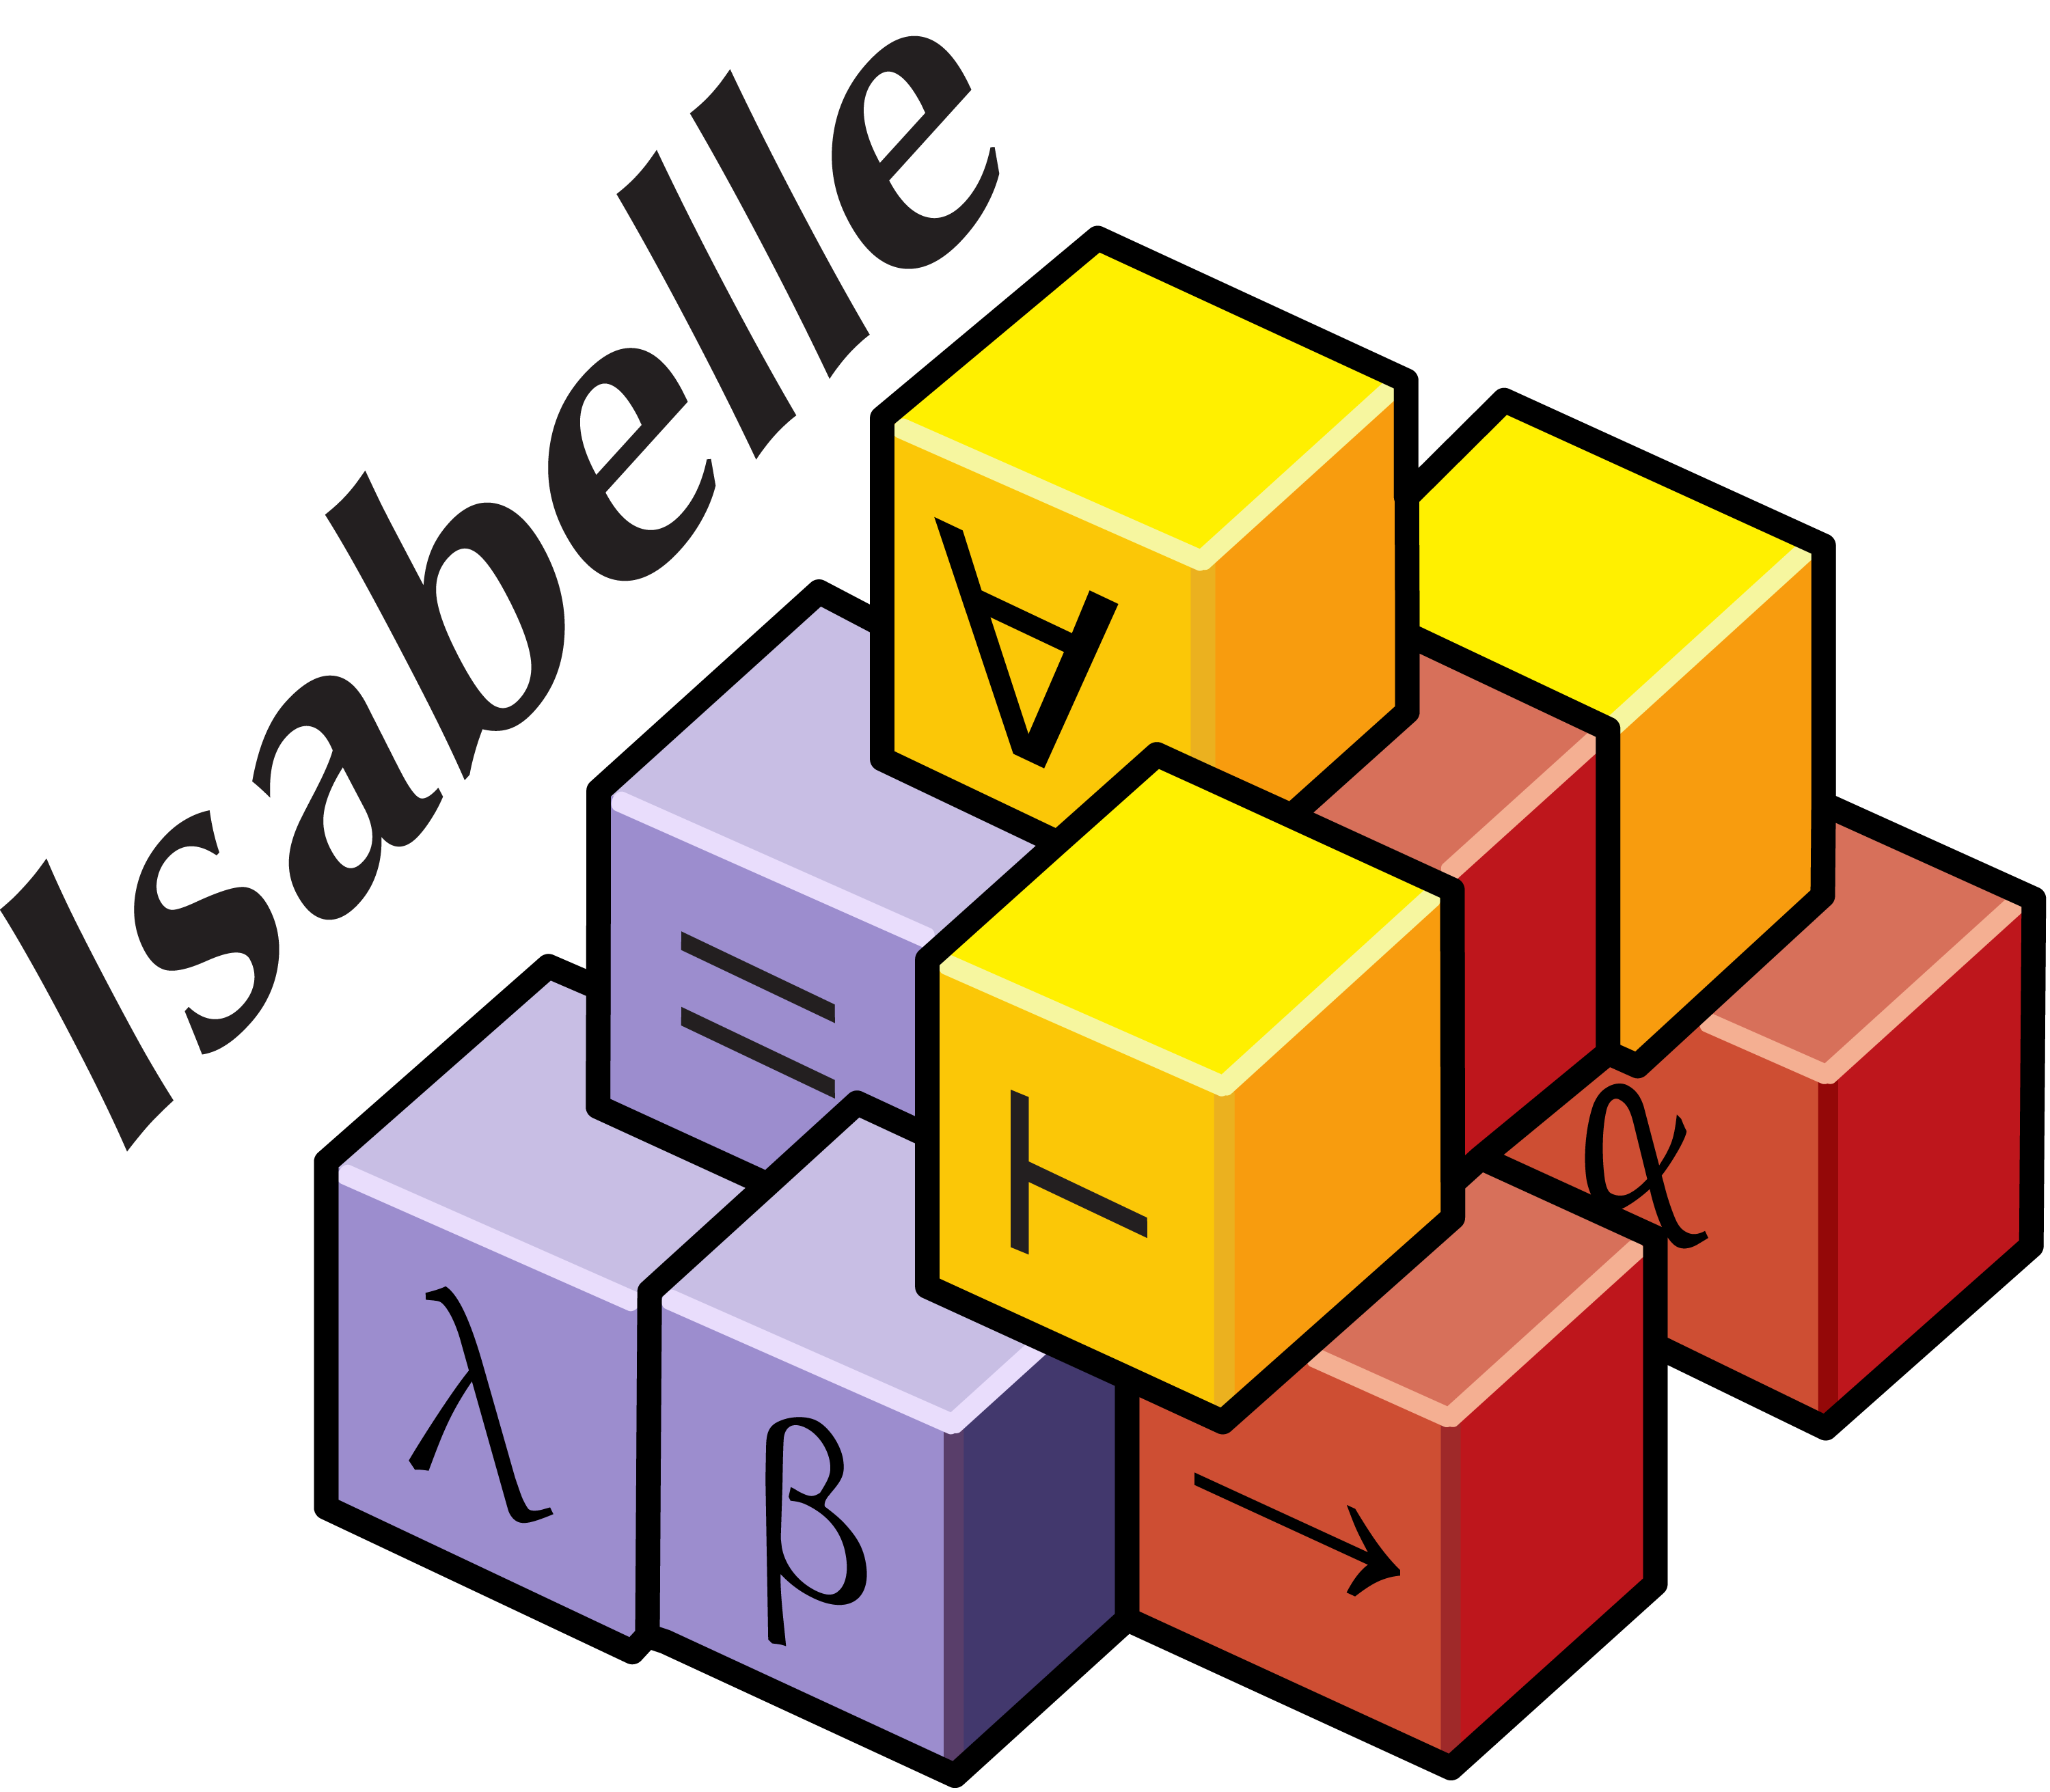
\includegraphics[height=1.5cm]{img/logoisabelle.png}
        \vfill
    \end{center}
    \begin{center}
        
        \textbf{Final year intership report}
        \vfill

        \large{\textbf{Verification in Isabelle/HOL of Hopcroft's algorithm for minimizing DFAs including runtime analysis}}
    \end{center}
    
    \vfill
    
    \begin{center}
        \textbf{Vincent Trélat}\\
        \vspace{1cm}
        \textit{\today}
    \end{center}
    \vfill
    \begin{center}
        
\includegraphics[height=1.2cm]{img/logoGE.png}
        \hfill
        
\includegraphics[height=1.2cm]{img/logoUL.png}
    \end{center}
\end{titlepage}

\tableofcontents

\pagebreak

\section{Introduction}

The algorithm was first presented in John E.\ Hopcroft's original 1971 paper \cite{Hop71} as a formal algorithm. This algorithm is presented in Algorithm~\ref{alg:original} with only slight changes in the notations.

\begin{algorithm}[H]
\SetAlgoLined
\caption{Hopcroft's original formal algorithm}
\label{alg:original}
\KwData{\textbf{Input:} a finite DFA $\mathcal{A} = (\mathcal{Q}, \Sigma, \delta, q_0, \mathcal{F})$}
\KwResult{\textbf{Output:} the equivalence class of $\mathcal{Q}$ under state equivalence}
$\delta^{-1}(q, a) := \{t \in \mathcal{Q}\ |\ \delta(t, a) = q\}$ for all $q \in \mathcal{Q}$ and $a \in \Sigma$ \;
$P_1 := \mathcal{F}$; $P_2 := \mathcal{Q} \setminus \mathcal{F}$;\\ $a_i := \{q \in P_i \ | \ \delta^{-1}(q, a) \neq \varnothing \}$ for all $i \in \{1, 2\}$ and $a \in \Sigma$ \;
$k := 3$ \;
For all $a \in \Sigma$, $L_a := \underset{0 \leq i < k}{\operatorname*{arg\,min}}\ \left| a_i \right|$ \;
\While{$\exists a \in \Sigma, L_a \neq \varnothing$}{
    Pick $a \in \Sigma$ such that $L_a \neq \varnothing$ and $i \in L_a$ \;
    $L_a := L_a \setminus \{i\}$ \;
    \ForAll{$j < k, \exists q \in P_j, \delta(q, a) \in a_i$}{
        $P'_j := \{t \in \mathcal{Q}\ |\ \delta(t, a) \in a_i \}$ and $P''_j := P_j \setminus P'_j$ \;
        $P_j := P'_j$ and $P_{k} := P''_j$; construct $a_j$ and $a_k$ for all $a \in \Sigma$ accordingly \;
        For all $a \in \Sigma$, $L_a := \begin{cases}
        L_a \cup \{j\} & \text{if $j \notin L_a \land \left| a_j \right| \leq \left| a_k \right|$} \\
        L_a \cup \{k\} & \text{otherwise}
        \end{cases}$ \;
        $k := k + 1$ \;
    }
}
\end{algorithm}

Today, the algorithm is usually given in a more mathematical way\footnote{see for example \cite{esparza2023automata}}, as in Algorithm~\ref{alg:modern}.

\begin{algorithm}[H]
\SetAlgoLined
\caption{Hopcroft's algorithm in modern notations}
\label{alg:modern}
\KwData{\textbf{Input:} a finite DFA $\mathcal{A} = (\mathcal{Q}, \Sigma, \delta, q_0, \mathcal{F})$}
\KwResult{\textbf{Output:} the language partition $P_\ell$}
\eIf{$\mathcal{F} = \varnothing \lor \mathcal{Q} \setminus \mathcal{F} = \varnothing$}{
    \Return $\mathcal{Q}$
}{
    $P := \{ \mathcal{F}, \mathcal{Q} \setminus \mathcal{F} \}$ \;
    $\mathcal{W} := \{ (a, \min \{ \mathcal{F}, \mathcal{Q} \setminus \mathcal{F}\}, a \in \Sigma \}$ \;
    \While{$\mathcal{W} \neq \varnothing$}{
        Pick $(a, B')$ from $\mathcal{W}$ \;
        \ForAll{$B \in P$}{
            Split $B$ with $(a, B')$ into $B_0$ and $B_1$ \;
            $P := (P \setminus \{B\}) \cup \{B_0, B_1\}$ \;
            \ForAll{$b \in \Sigma$}{
                \eIf{$(b, B \in \mathcal{W})$}{
                    $\mathcal{W} := (\mathcal{W} \setminus \{(b, B)\}) \cup \{(b, B_0), (b, B_1)\}$ \;
                }{
                    $\mathcal{W} := \mathcal{W} \cup \{(b, \min \{ B_0, B_1 \})\}$ \;
                }
            }
        }
    }
}

\end{algorithm}

\section{Proof of correctness}
\section{Time complexity analysis}

% \printglossary[type=\acronymtype]

% \addcontentsline{toc}{section}{CV}
% \includepdf{cv.pdf}

\pagebreak
% bibliography
\bibliographystyle{alpha}
\bibliography{ref}

\end{document}